\documentclass[xcolor={cmyk}]{beamer}
\usepackage[utf8]{inputenc}
\usepackage[T1]{fontenc}
\usepackage[english]{babel}
\usepackage{verbatim}
\graphicspath{{./pics/}}

\title{4G LTE CoMP, Coordinated Multipoint}
\subtitle{4th Semester Institute Project}
\author[Matthis Dirksen]{\tiny Leonhard Hetz \and Philipp Braun \and Carmine Bianco \and Alissa Wenzel \and Matthis Dirksen}
\date{July 21, 2016}

% Select theme
\usetheme[english]{RWTH_Ti}
\setbeamercolor*{block body}{bg = white}

\begin{document}

% Titlepage
\frame[plain]{\titlepage}

% Template for the slides: 
\begin{comment}
 
 \begin{frame}{4G LTE CoMP, Coordinated Multipoint}{4th Semester Institute Project}
	 \begin{block}{...}
	
	 \end{block}
 \end{frame}
 
 \end{comment}

% Content Slide
\begin{frame}{Overview}
	\begin{block}{Content}
		\begin{columns}
			\begin{column}{.9\textwidth}
				\begin{itemize}
					\item Motivation
					\item Background
					\item System Model
					\item Simulation
					\item Evaluation
					\item Conclusions
					\item References
				\end{itemize}
			\end{column}
		\end{columns}
	\end{block}
\end{frame}

% Content Slide highlight Motivation 
\begin{frame}{Overview}
	\begin{block}{Content}
		\begin{columns}
			\begin{column}{.9\textwidth}
				\begin{itemize}
					\item \textbf{\emph{Motivation}}
					\item Background
					\item System Model
					\item Simulation
					\item Evaluation
					\item Conclusions
					\item References
				\end{itemize}
			\end{column}
		\end{columns}
	\end{block}
\end{frame}

% Motivation Slide
 \begin{frame}{Motivation}
	 \begin{block}{}
	 	\begin{columns}
			\begin{column}{.9\textwidth}
				\begin{itemize}
					\item Due to the network densification plans, interference will substantially increase. Interference management will play an important role in future networks
					\item Mainly cell edge users suffer from interference
					\item Goal is to improve performance via interference management schemes - such as CoMP 
					\item CoMP is a broad category of cooperation in the network with the aim of enhancing user performance
				\end{itemize}
			\end{column}
		\end{columns}
	 \end{block}
 \end{frame}
 
 % Content Slide highlight Background 
\begin{frame}{Overview}
	\begin{block}{Content}
		\begin{columns}
			\begin{column}{.9\textwidth}
				\begin{itemize}
					\item Motivation
					\item \textbf{\emph{Background}}
					\item System Model
					\item Simulation
					\item Evaluation
					\item Conclusions
					\item References
				\end{itemize}
			\end{column}
		\end{columns}
	\end{block}
\end{frame}

% BACKGROUND SLIDES

% TO DO
% - JT too complicated, higher backhaul
% - explain backhaul?

% General information of research
 \begin{frame}{Background}
	 \begin{block}{Overview on research}
	 	\begin{columns}
			\begin{column}{.9\textwidth}
				\begin{itemize}
					\item Papers on LTE-A, Joint Transmission, Beamforming and CoMP in general
					\item Reference: MATLAB-based down-
link physical-layer simulator for LTE (Mehlführer, C., 2009)
					\begin{itemize}
						\item MATLAB-based downlink physical-layer simulator for LTE
						\item Covering Multi-Cell Multi-User simulation scenarios $\rightarrow$ most realistic
					\end{itemize}
				\end{itemize}
			\end{column}
		\end{columns}
	 \end{block}
 \end{frame}
 
 
 % Scheduling
 \begin{frame}{Background}
 	\begin{block}{Scheduling}
		\begin{columns}
			\begin{column}{.9\textwidth}
				\begin{itemize}
					\item Assignment of resource blocks (RB) to each user
					\item i.e. Round Robin (timeslots divided equally between users)
					\item Dynamic scheduling: mapping RBs to users based on different criteria
				\end{itemize}
			\end{column}
		\end{columns}
	 \end{block}
 \end{frame}

% SINR
 \begin{frame}{Background}
 	\begin{block}{Channel model}
		\begin{columns}
			\begin{column}{.9\textwidth}
				\begin{itemize}
					\item Signal-to-interference-plus-noise ratio $\rightarrow$ Description of the channel
					\begin{equation*}
\frac{P_j*(h_j*w_j)^{2}}{\sum (h_i*w_i)^{2}*P_i+(\sigma_N)^{2}}
					\end{equation*}
					\begin{itemize}
						\item P\textsubscript{j} - Power of signal
						\item h\textsubscript{j} - Channel
						\item w - Precoding matrix
						\item p\textsubscript{i} - Power of interference
						\item sigma\textsubscript{N} - Noise
					\end{itemize}
					\item Used to determine signal quality
					\item Block-fading channel to reduce complexity
				\end{itemize}
			\end{column}
		\end{columns}
	 \end{block}
 \end{frame}

% CQI and channel modulation
 \begin{frame}{Background}
 	\begin{block}{User feedback (CSI)}
		\begin{columns}
			\begin{column}{.9\textwidth}
				\begin{itemize}
					\item Channel Quality Indicator
					\item Determines modulation
					\begin{itemize}
						\item Transfer block size (TBS)
						\item Resource blocks for users
					\end{itemize}
					\item Depends on SINR
					\item CSI includes CQI, PMI, RI. CQI depends on SINR, PMI and RI depends on beamforming
				\end{itemize}
			\end{column}
		\end{columns}
	 \end{block}
 \end{frame}

 
 % CoMP - overview
 \begin{frame}{Background - CoMP}
 	\begin{block}{Overview}
		\begin{columns}
			\begin{column}{.9\textwidth}
				\begin{itemize}
					\item LTE Advanced: major enhancement of the LTE standard
					\item CoMP: Coordinate MultiPoint operation
					\begin{itemize}
						\item Refers to wide range of interference management techniques
						\item Dynamic coordination or transmission and reception with multiple geographically separated eNBs (base stations)
						\item Goal: enhancing overall system performance, more effective use of resources, improved end user service quality (especially at the cell edges)
					\end{itemize}
				\end{itemize}
			\end{column}
		\end{columns}
	 \end{block}
 \end{frame}
 
% CoMP - Major Categories
 \begin{frame}{Background - CoMP}
 	\begin{block}{Major categories}
		\begin{columns}
\column{.5\textwidth}
			Joint Processing (JP)
				\begin{itemize}
					\item Joint Transmission (JT)
					\item Dynamic Point Selection (DPS)
					\begin{itemize}
						\item With muting
						\item Without muting
					\end{itemize}
				\end{itemize}			
			\column{.5\textwidth}
				Coordinated Scheduling (CS) / Coordinated Beamforming (CB)
		\end{columns}
		 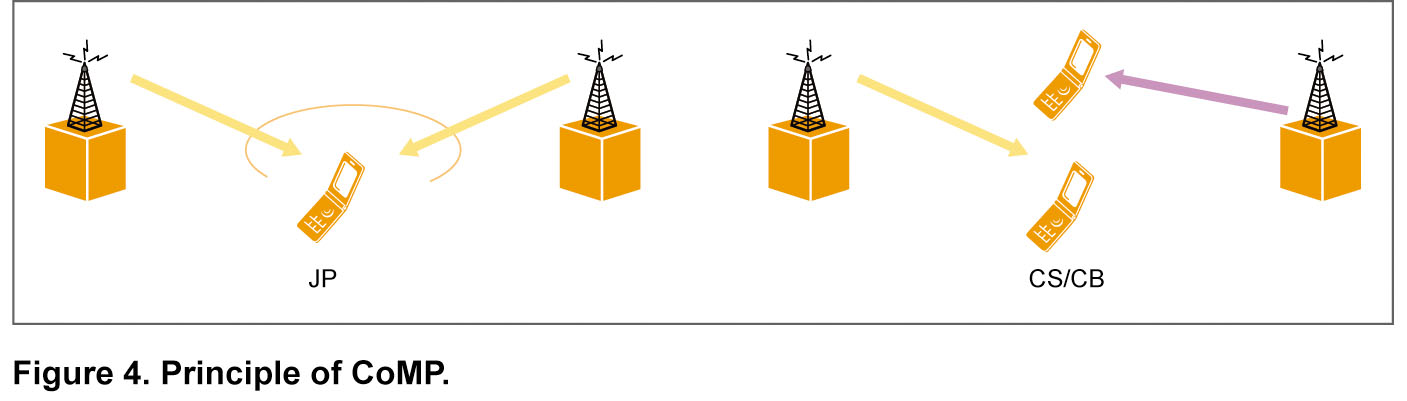
\includegraphics[width=\linewidth,height=\textheight,keepaspectratio]{W020101021303791421974.jpg}
	 \end{block}
 \end{frame}
 
 % Coordinated Scheduling
 \begin{frame}{Background - CoMP}
 	\begin{block}{Coordinated Scheduling (CS)}
		\begin{columns}
			\begin{column}{.9\textwidth}
				\begin{itemize}
					\item Data available at one node
					\item Transfered packets do not overlap in time
					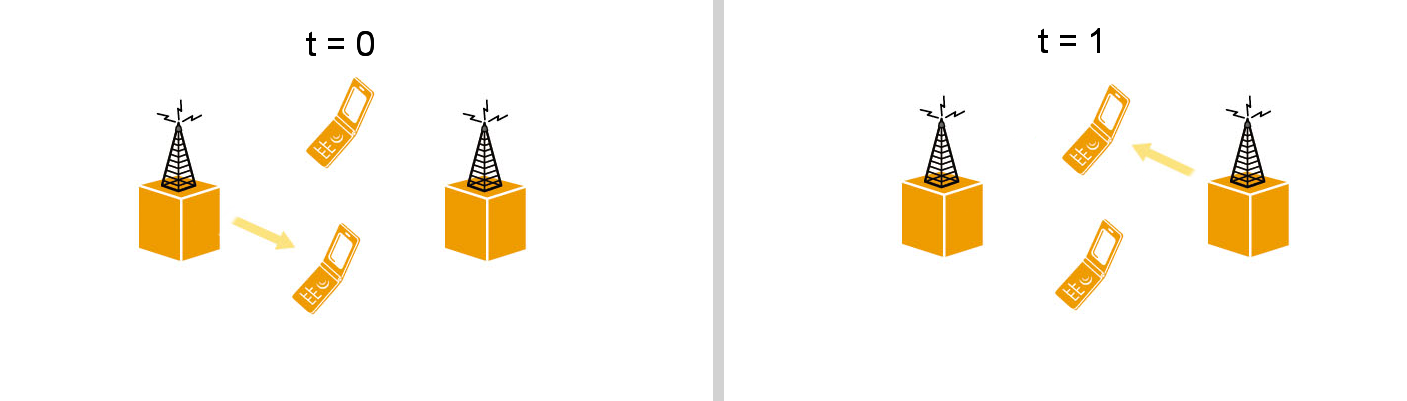
\includegraphics[width=\linewidth,height=\textheight,keepaspectratio]{GrafikCS.png}
				\end{itemize}
			\end{column}
		\end{columns}
	 \end{block}
 \end{frame}

% Dynamic Point Selection
 \begin{frame}{Background - CoMP}
 	\begin{block}{Dynamic Point Selection (DPS)}
		\begin{columns}
			\begin{column}{.9\textwidth}
				\begin{itemize}
					\item Data usually available at several nodes
					\item User decides per packet which base station is best
					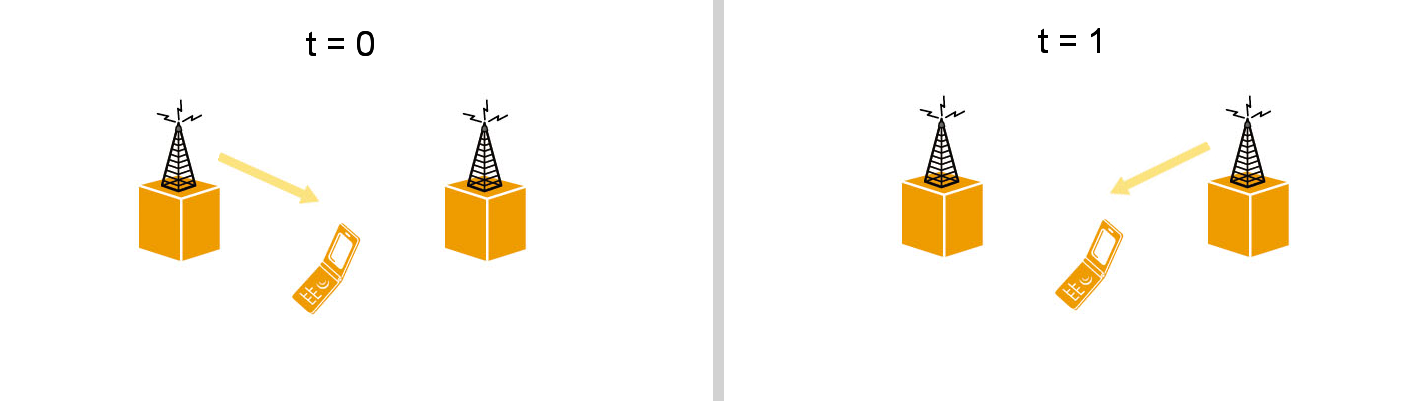
\includegraphics[width=\linewidth,height=\textheight,keepaspectratio]{GrafikDPS.png}
				\end{itemize}
			\end{column}
		\end{columns}
	 \end{block}
 \end{frame}
 
 % Content Slide highlight System Model 
\begin{frame}{Overview}
	\begin{block}{Content}
		\begin{columns}
			\begin{column}{.9\textwidth}
				\begin{itemize}
					\item Overview
					\item Background
					\item \textbf{\emph{System Model}}
					\item Simulation
					\item Evaluation
					\item Conclusions
					\item References
				\end{itemize}
			\end{column}
		\end{columns}
	\end{block}
\end{frame}

% System Model Slide
 \begin{frame}{System Model}
	 \begin{block}{Assumptions}
	 	\begin{columns}
			\begin{column}{.9\textwidth}
				\begin{itemize}
					\item Geographical Location of UE is known
					\item UE does not move so no Doppler effect, studying slow fading
					\item CQI, PMI, RI are randomly generated
					\begin{itemize}
						\item PMI depends on generated CQI
					 \end{itemize}
					\item Fixed number of UEs in a simulation
					\item Mean values of the Rayleigh distribution (provided from 3GPP)
					\item Basestations are created in a hexagonal layout
				\end{itemize}
			\end{column}
		\end{columns}
	 \end{block}
 \end{frame}
 
% System Model Slide
 \begin{frame}{System Model}
	 \begin{block}{Programming}
	 	\begin{columns}
			\begin{column}{.9\textwidth}
				\begin{itemize}
					\item Classes providing main functionality: Central Unit, Base Station, User Entity, Channel
					\item Classes providing background data and auxiliary functions: TBS, Helpers, Params, Precoding Matrix (PMI)
				\end{itemize}
			\end{column}
		\end{columns}
	 \end{block}
 \end{frame}
 
   % Channel Simulation Results
  \begin{frame}{4G LTE CoMP, Coordinated Multipoint}{4th Semester Institute Project}
	 \begin{block}{CQI and Spectral Efficiency}
		 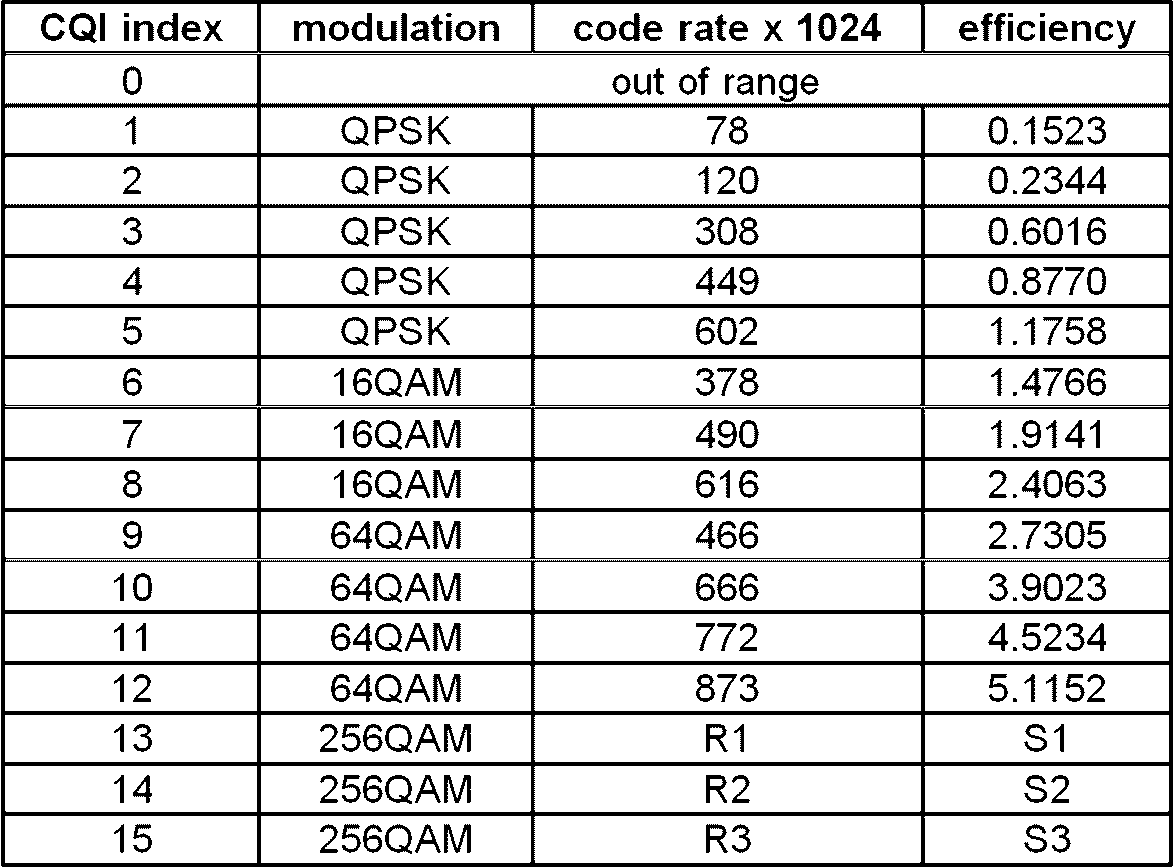
\includegraphics[width=\linewidth]{cqi.png}
	 \end{block}
 \end{frame}
 
 % Details on our Classes
  \begin{frame}{System Model}
	 \begin{block}{Classes providing main functionality}
	 	\begin{columns}
			\begin{column}{.9\textwidth}
				\begin{itemize}
					\item Central Unit
					\begin{itemize}
						\item Coordinates all base stations 
					\end{itemize}
					\item Base Station
					\begin{itemize}
						\item Matches subcarriers to connected users, calculates modulation
					\end{itemize}
					\item User Entity
					\begin{itemize}
						\item Returns feedback to each base station
					\end{itemize}
					
					\item Channel
					\begin{itemize}
						\item Certain frequency and amount of subcarriers
						\item Friis equation for calculation of path loss
						\item Model - Rayleigh channel
					\end{itemize}
				\end{itemize}
			\end{column}
		\end{columns}
	 \end{block}
 \end{frame}
 
  % Details on our Classes
  \begin{frame}{System Model}
	 \begin{block}{Slow versus Fast Fading}
	 	\begin{columns}
			\begin{column}{.9\textwidth}
				\begin{itemize}
					\item Slow Fading
					\begin{itemize}
						\item Coherence time of the channel is large relative to the delay requirement of the application
						\item Amplitude and Phase Change imposed by the channel can be considered roughly constant
					\end{itemize}
					\item Fast Fading
					\begin{itemize}
						\item Coherence time of the channel is short relative to the delay requirement of the application
						\item Amplitude and Phase Change imposed by the channel varies considerably over the period of use
					\end{itemize}
					
					
					\item Block Fading chosen for simplicity
				\end{itemize}
			\end{column}
		\end{columns}
	 \end{block}
 \end{frame}
 
  % Channel Simulation Results
  \begin{frame}{4G LTE CoMP, Coordinated Multipoint}{4th Semester Institute Project}
	 \begin{block}{Rayleigh Channel Simulation}
		 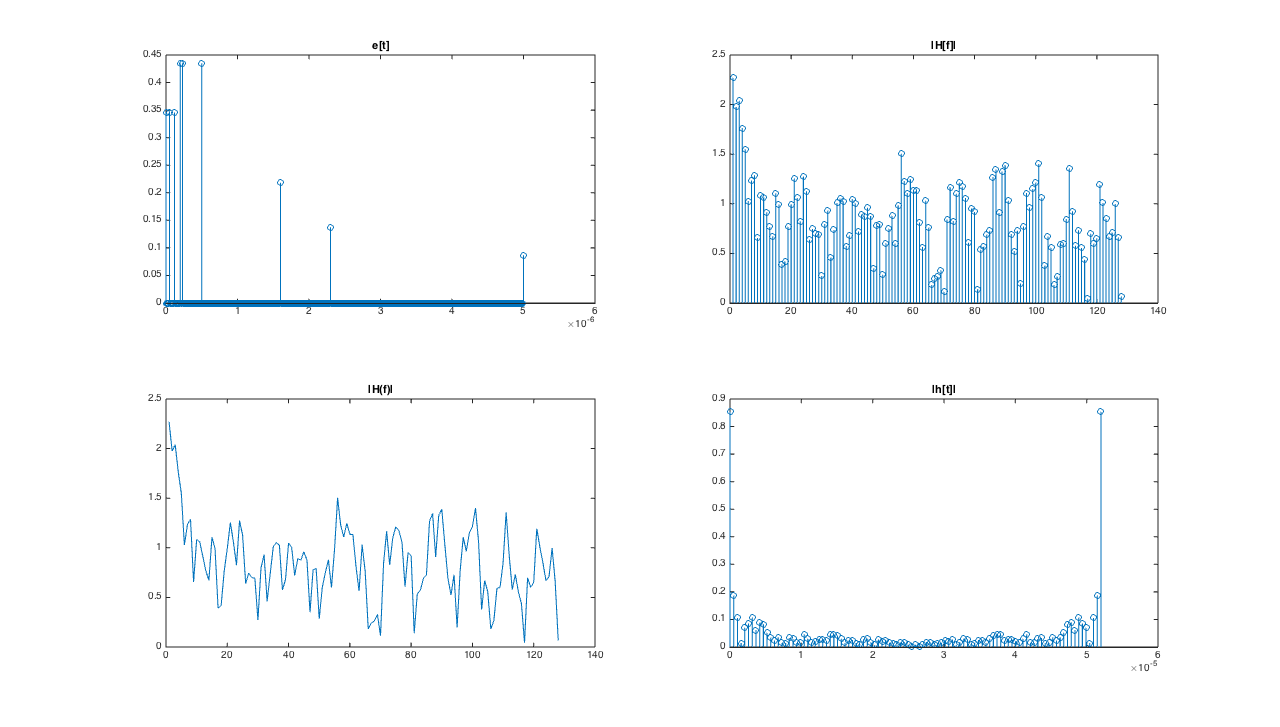
\includegraphics[width=\linewidth,height=\textheight,keepaspectratio]{channel.png}
	 \end{block}
 \end{frame}
 
 % Slide with overview of the classes
  \begin{frame}{4G LTE CoMP, Coordinated Multipoint}{4th Semester Institute Project}
	 \begin{block}{Class Overview}
		 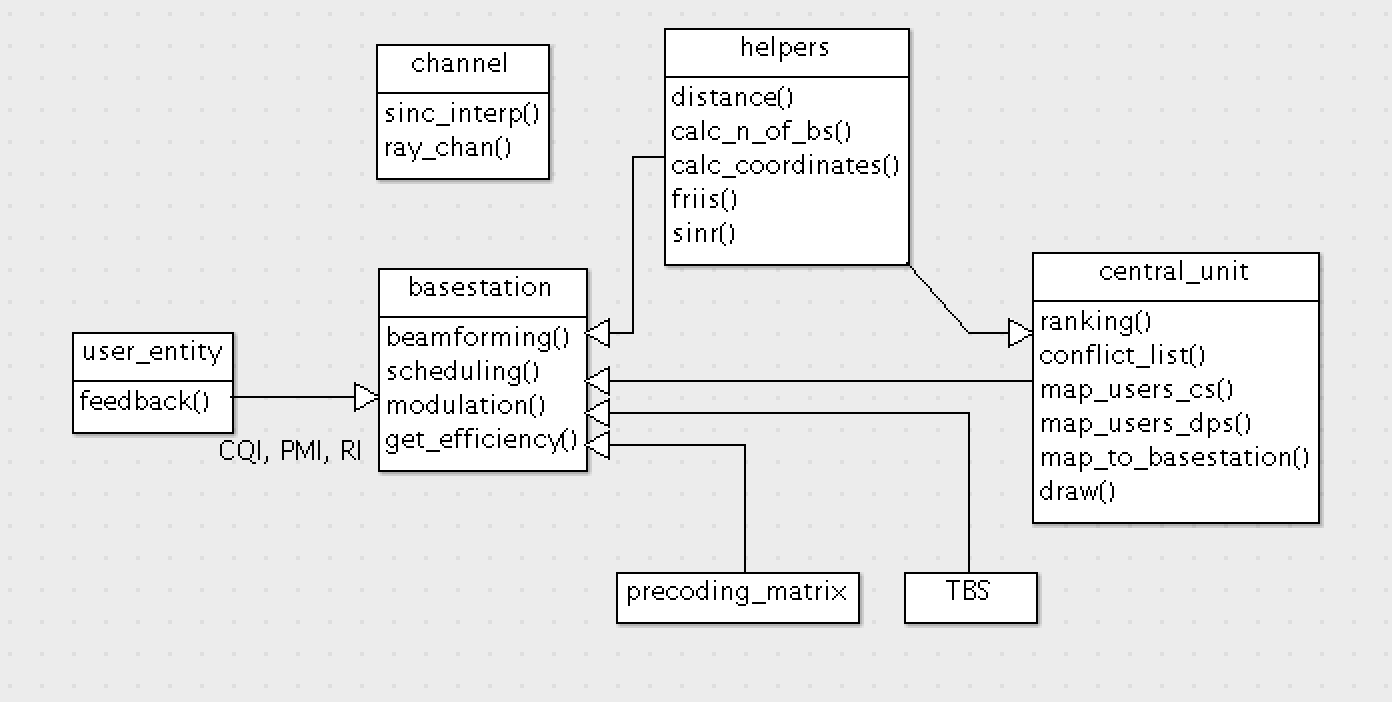
\includegraphics[width=\linewidth,height=\textheight,keepaspectratio]{klassen.png}
	 \end{block}
 \end{frame}

% Friis Equation
  \begin{frame}{4G LTE CoMP, Coordinated Multipoint}{4th Semester Institute Project}
	 \begin{block}{Friis Equation}
		\begin{equation*}
			P_r = P_t + G_t + G_r + 20 log_{10}(\frac{\lambda}{4 \pi R})
		\end{equation*}
		\begin{itemize}
			\item G - Antenna Gains
			\item P - Received/Transmitted Power
			\item $\lambda$ - Wavelength
			\item R - Distance between Antennas
			\item Units in dB
		\end{itemize}
	 \end{block}
 \end{frame}

  % SINR Profile
  \begin{frame}{4G LTE CoMP, Coordinated Multipoint}{4th Semester Institute Project}
	 \begin{block}{SINR Profile}
		 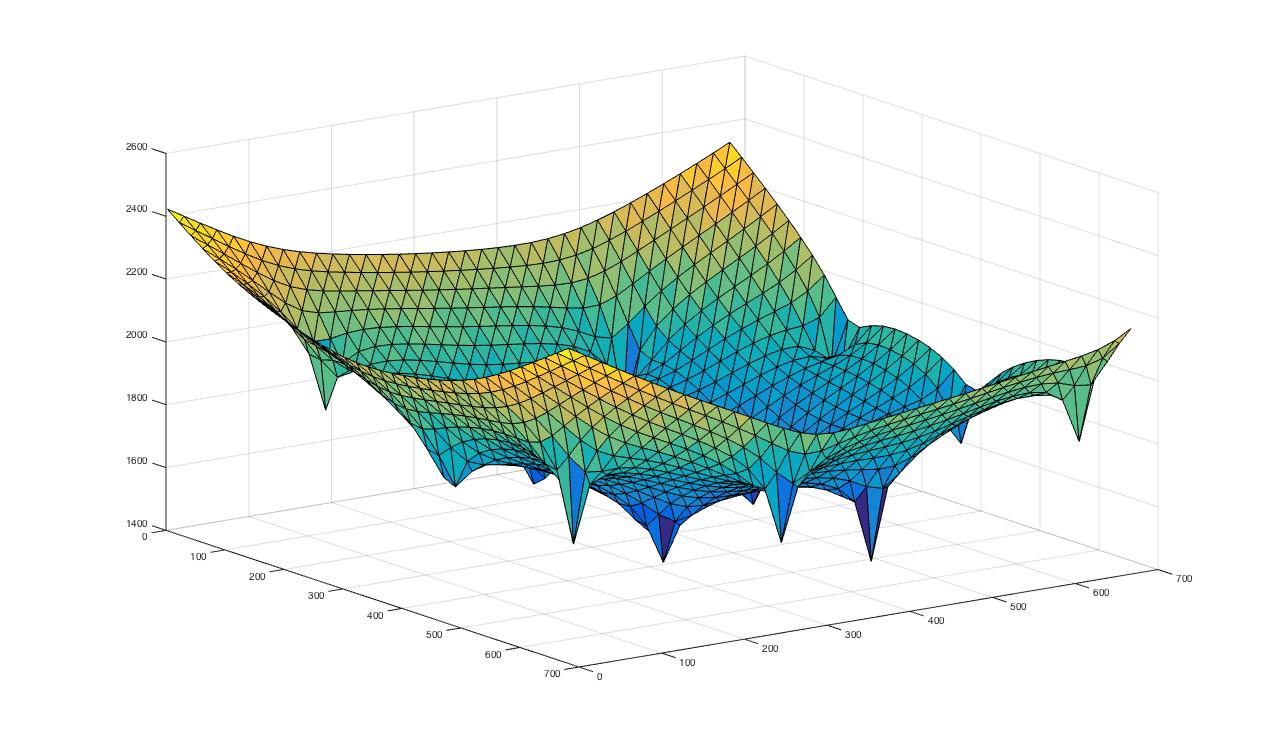
\includegraphics[width=\linewidth,height=\textheight,keepaspectratio]{sinr.jpg}
	 \end{block}
 \end{frame}
 
 % Content Slide highlight Simulation
\begin{frame}{Overview}
	\begin{block}{Content}
		\begin{columns}
			\begin{column}{.9\textwidth}
				\begin{itemize}
					\item Motivation
					\item Background
					\item System Model
					\item \textbf{\emph{Simulation}}
					\item Evaluation
					\item Conclusions
					\item References
				\end{itemize}
			\end{column}
		\end{columns}
	\end{block}
\end{frame}

% Simulation Slide
% What is it able to do?
 \begin{frame}{Simulation}
	 \begin{block}{Main characteristics}
	 	\begin{columns}
			\begin{column}{.9\textwidth}
				\begin{itemize}
					\item Flexibility
					\item Modularity
					\item Simulation Process
					\begin{itemize}
						\item Initialization
						\item Simulation Cycle
						\begin{itemize}
							\item mapping of users to basestations
							\item assignment of resource blocks to users
							\item calculation of the best modulation and coding scheme
					 	\end{itemize}
					 \end{itemize}
					
				 \end{itemize}
			\end{column}
		\end{columns}
	 \end{block}
 \end{frame}
 
% simulation slide II
 \begin{frame}{Simulation}
 \begin{block}{Simulation DPS I}
 
 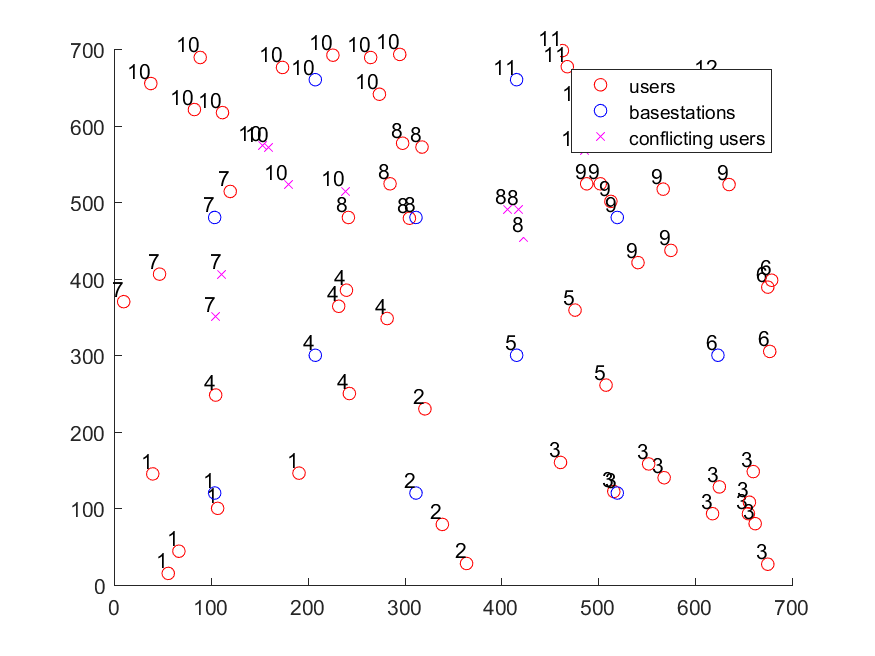
\includegraphics[width=\linewidth,height=\textheight,keepaspectratio]{MapPlotDPS1.png}
 \end{block}
 \end{frame}
 
 % simulation slide III
 \begin{frame}{Simulation}
 \begin{block}{Simulation DPS II}
 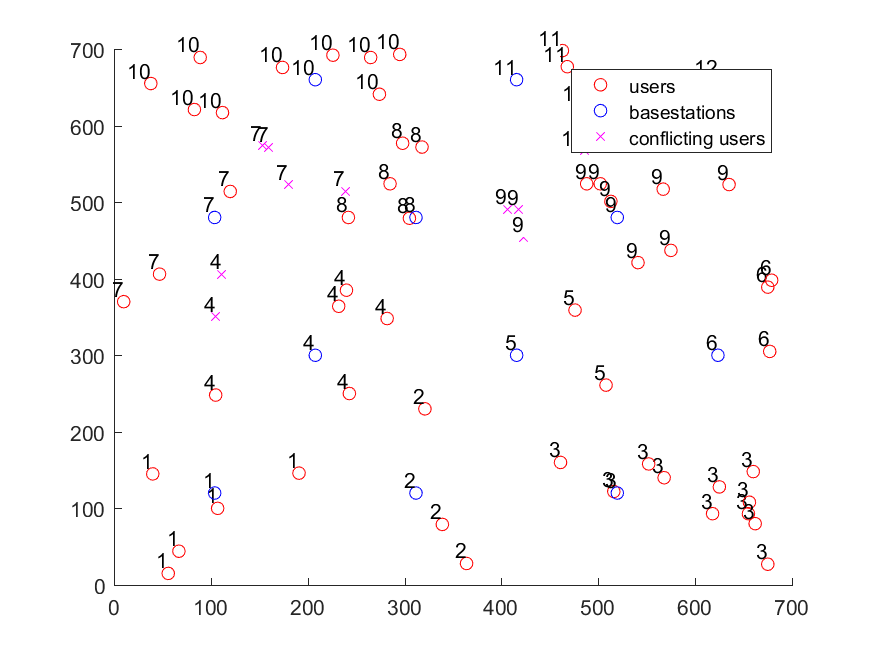
\includegraphics[width=\linewidth,height=\textheight,keepaspectratio]{MapPlotDPS2.png}
 \end{block}
 \end{frame}
 
 % simulation slide II
 \begin{frame}{4G LTE CoMP, Coordinated Multipoint}{4th Semester Institute Project}
 \begin{block}{Simulation CS I}
 
 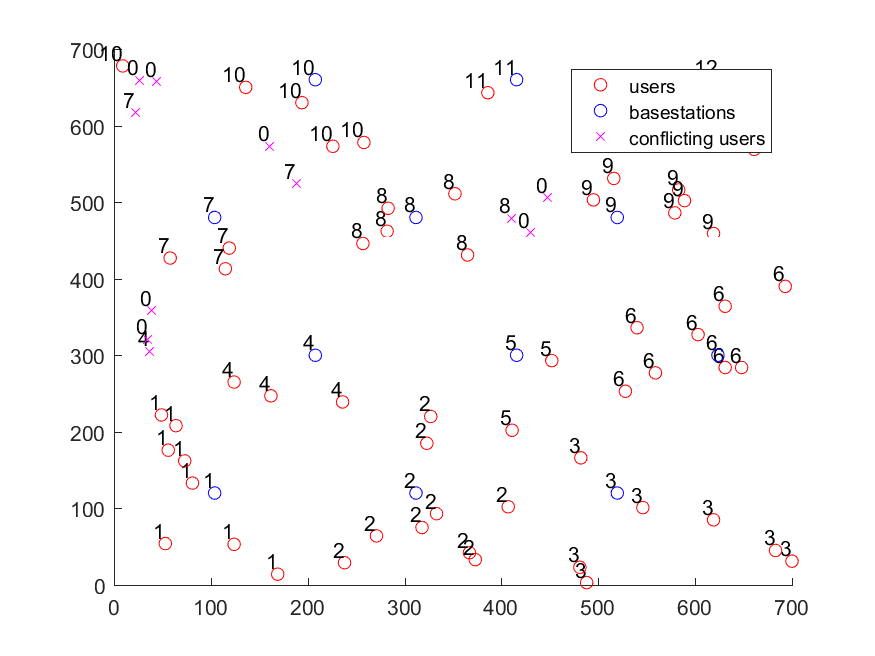
\includegraphics[width=\linewidth,height=\textheight,keepaspectratio]{MapPlotCS1.png}
 \end{block}
 \end{frame}
 
 % simulation slide III
 \begin{frame}{Simulation}
 \begin{block}{Simulation CS II}
 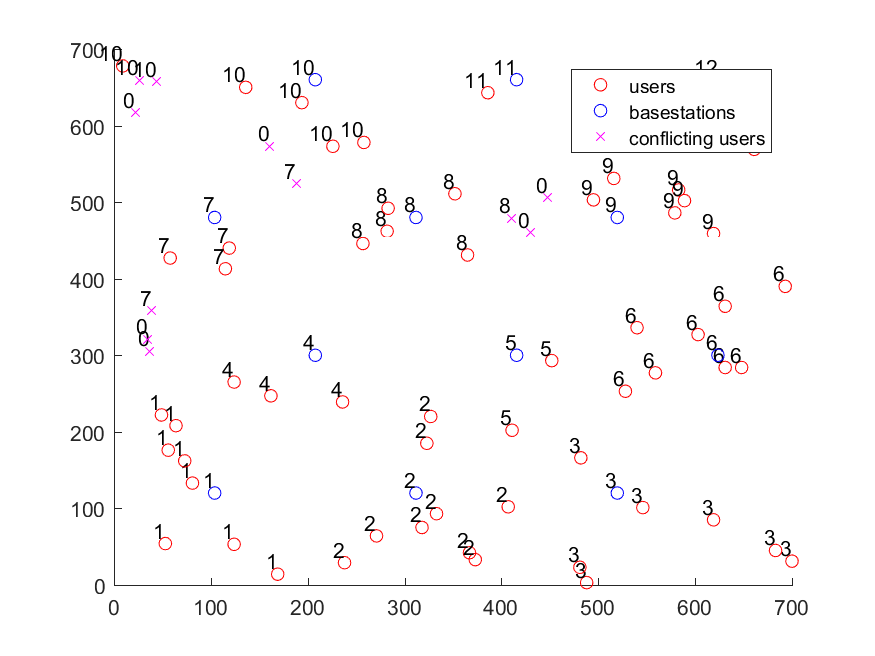
\includegraphics[width=\linewidth,height=\textheight,keepaspectratio]{MapPlotCS2.png}
 \end{block}
 \end{frame}
 
 % Content Slide highlight Evaluation
\begin{frame}{Overview}
	\begin{block}{Content}
		\begin{columns}
			\begin{column}{.9\textwidth}
				\begin{itemize}
					\item Motivation
					\item Background
					\item System Model
					\item Simulation
					\item \textbf{\emph{Evaluation}}
					\item Conclusions
					\item References
				\end{itemize}
			\end{column}
		\end{columns}
	\end{block}
\end{frame}
 
% Evaluations Slide
% Simulation with and without Comp
% why should you use CoMP
 \begin{frame}{Evaluation}
	 \begin{block}{}
 \begin{columns}
			\begin{column}{.9\textwidth}
				\begin{itemize}
					\item 5000 Simulation Cycles
					\item 70 User Entities, 12 Basestations
				\end{itemize}
			\end{column}
		\end{columns} 
		\end{block}\ \\
	 \begin{tabular}{|l|l|l|l|}
	 \hline
	 & without CoMp & DPS & CS \\ \hline
	 users in conflict & 19.65\% & 19.78\% & 19.67\% \\ \hline
	 unassigned users & 0\% & 0\% & 10.5\% \\ \hline
	 average backhaul[bit/s] & 78081 & 90791 & 77317 \\ \hline
	 additional backhaul & +0\% & +16.28\% & -0.98\% \\ \hline
	
	 \end{tabular}

 \end{frame}
 
 % Slide on why to use CoMP
 \begin{frame}{Evaluation}
	 \begin{block}{Advantages}
	 	\begin{columns}
			\begin{column}{.9\textwidth}
				\begin{itemize}
					\item Less interference at cell edges, thus better SINR performance.
					\item Utilization of different subcarriers inside conflict zones avoids interference
				\end{itemize}
			\end{column}
		\end{columns}
	 \end{block}
	 \begin{block}{Disadvantages}
	 	\begin{columns}
			\begin{column}{.9\textwidth}
				\begin{itemize}
					\item Complexity of algorithms
					\item Infeasibility with restricted backhauls
					\item Bigger signaling overhead between users and base stations
					\item More frequent communication with the CU --> bigger backhaul needed
				\end{itemize}
			\end{column}
		\end{columns}
	 \end{block}
 \end{frame}

 
  % Content Slide highlight Conclusions
\begin{frame}{Overview}
	\begin{block}{Content}
		\begin{columns}
			\begin{column}{.9\textwidth}
				\begin{itemize}
					\item Motivation
					\item Background
					\item System Model
					\item Simulation
					\item Evaluation
					\item \textbf{\emph{Conclusions}}
					\item References
				\end{itemize}
			\end{column}
		\end{columns}
	\end{block}
\end{frame}

% Conclusions Slide
\begin{frame}{Summary}
	\begin{block}{}
		\begin{columns}
			\begin{column}{.9\textwidth}
				\begin{itemize}
					\item Main functionalities for a LTE-Advanced simulator implemented
					\begin{itemize}
						\item Implementation of \textbf{Coordinated Scheduling} and \textbf{Dynamic Point Selection}
						\item Comparison with system behaviour without CoMP
					\end{itemize}
					\item Advantages of CoMP mainly for users at cell edges
					\begin{itemize}
						\item Profitability vs backhaul/signaling trade-offs should be evaluated on a case-by-case basis
						\item Possible solution: activating Coordinated Multipoint only as a certain conflict density in the simulated environment is reached
					\end{itemize}
				\end{itemize}
			\end{column}
		\end{columns}
	\end{block}
\end{frame}

%Conclusions #2: which (factual) goals did we reach in the project?
\begin{frame}{Summary}
	 \begin{block}{Project goals reached}
	 	\begin{columns}
			\begin{column}{.9\textwidth}
				\begin{itemize}
					\item Analysis of behaviour of frequency flat, slow fading channels
					\item Differences between SISO and MIMO channel models and their implications
					\item Criteria for estabishling a state of conflict between different user entities
					\item Choice of channel modulation based upon generated feedback
					\item Allocating users to base stations according to selected CoMP scheme
				\end{itemize}
			\end{column}
		\end{columns}
	 \end{block}
 \end{frame}

%Conclusions #3: what did we learn (soft skills et al.) by working on this project (on two slides)

\begin{frame}{Summary}
	 \begin{block}{Learning goals reached}
	 	 \hspace*{.1\linewidth}\begin{minipage}{.8\linewidth}
    		\begin{block}{Programming}
      			\begin{itemize}
      				\item \textbf{Object-oriented programming} on MATLAB
      				\item Graphical representation of simulation results
      				\item Working with parameter files/external files (e.g. precoding matrix) and already existing MATLAB libraries
      				\item Making model abstractions while maintaining accuracy
      			\end{itemize}
    		\end{block}
    	\end{minipage}
	 \end{block}	 
 \end{frame}

\begin{frame}{Summary}
	 \begin{block}{Learning goals reached}
    	\hspace*{.1\linewidth}\begin{minipage}{.8\linewidth}
    		\begin{block}{Soft skills}
      			\begin{itemize}
      				\item Collection of preliminary informations through approach to English language scientific literature
      				\item Teamwork: weekly meetings and frequent contacts with the project supervisors
      				\begin{itemize}
      					\item Task division in the team according to current needs and time availability
      				\end{itemize}
      				\item Debugging and version control on GitHub
      				\item \LaTeX basics for the final presentation
      			\end{itemize}
    		\end{block}
    	\end{minipage}
	 \end{block}	 
 \end{frame}

%Last slide: possible expansions: what could still be done?
 \begin{frame}{Future work}
	 \begin{block}{What comes next?}
	 	\begin{columns}
			\begin{column}{.9\textwidth}
				\begin{itemize}
					\item Implementation of other CoMP schemes, e.g. coordinated beamforming and joint transmission
					\item Different channel models (e.g. \textit{fast fading} channels)
					\item Optimization of CoMP techniques
					\begin{itemize}
						\item Different allocation of implementation stages between CU and BS
						\item Other scheduling patterns (currently implemented: Round Robin)
					\end{itemize}
					\item Implementation of different environment setups and parameters
				\end{itemize}
			\end{column}
		\end{columns}
	 \end{block}
 \end{frame}


  % Content Slide highlight References
\begin{frame}{Overview}
	\begin{block}{Content}
		\begin{columns}
			\begin{column}{.9\textwidth}
				\begin{itemize}
					\item Motivation
					\item Background
					\item System Model
					\item Simulation
					\item Evaluation
					\item Conclusions
					\item \textbf{\emph{References}}
				\end{itemize}
			\end{column}
		\end{columns}
	\end{block}
\end{frame}

% References Slide
% Papers etc.
 \begin{frame}{4G LTE CoMP, Coordinated Multipoint}{4th Semester Institute Project}
	 \begin{block}{References}
	 	\begin{columns}
			\begin{column}{.9\textwidth}
				\begin{itemize}
					\item Mehlführer, C. et al, 2009. Simulating The Long Term Evolution Physical Layer. Proc. 17th European Signal Processing Conference (EUSIPCO 2009), [online]
					\item Davydov, A. et al, 2013. Evaluation of Joint Transmission CoMP in C-RAN based LTE-A HetNets with Large Coordination Areas. Globecom 2013 Workshop.
					\item Hong, M. et al, 2012. Joint Base Station Clustering and Beamformer Design for Partial Coordinated Transmission in Heterogeneous Networks.
					\item Sawahashi, M. et al, 2010. Coordinated Multipoint Transmission/Reception Techniques For LTE-Advanced.
				\end{itemize}
			\end{column}
		\end{columns}
	 \end{block}
 \end{frame}
 
 % Last Slide
  \begin{frame}{4G LTE CoMP, Coordinated Multipoint}{4th Semester Institute Project}
	\begin{block}{Thank you for your attention!}
	\end{block}
 \end{frame}


\end{document}